% THIS IS SIGPROC-SP.TEX - VERSION 3.1
\documentclass{sig-alternate}

% Additional packages
\usepackage{graphicx}
\usepackage{color}
\usepackage{url}
\usepackage{algorithm}
\usepackage[noend]{algpseudocode}
\usepackage{amsmath}
%\usepackage{amsthm}
\usepackage{amsfonts}
\usepackage{amssymb}
\usepackage{booktabs}
\usepackage{multirow}
\usepackage{ifpdf}
% Custom commands
\usepackage{custom_commands}

%\newcommand{\note}[1]{\relax} %{\color{red}#1}}
\newcommand{\note}[1]{{\color{red}#1}}

\newcommand{\prg}[1]{\paragraph{#1}}
%\newcommand{\prg}[1]{\textbf{#1}}

\newcommand{\Siren}{\textsc{Siren}}
\newcommand{\ReReMi}{\textsc{ReReMi}}

\begin{document}
\special{papersize=8.5in,11in}
\setlength{\pdfpageheight}{11in}%{\paperheight}
\setlength{\pdfpagewidth}{8.5in}%{\paperwidth}


\title{Siren: An Interactive Tool for Mining and Visualizing Geospatial Redescriptions}
\subtitle{[Demo]}

\numberofauthors{2} 
\author{
% 1st. author
\alignauthor
Esther Galbrun\\
       \affaddr{Department of Computer Science}\\
       \affaddr{University of Helsinki, Finland}\\
       \email{galbrun@cs.helsinki.fi}
% 2nd. author
\alignauthor
Pauli Miettinen\\
       \affaddr{Max Plack Institute for Informatics}\\
       \affaddr{Saarbr{\"u}cken, Germany}\\
       \email{pmiettin@mpi-inf.mpg.de}
}

\maketitle
\begin{abstract}
  We present \Siren, an interactive tool for mining geospatial
  redescriptions.  Redescription mining is a powerful data analysis
  tool that aims at finding alternative descriptions of the same
  entities.  For example, in biology, an important task is to identify
  the bioclimatic constraints that allow some species to survive, that
  is, to describe geographical regions in terms of both their
  bioclimatic conditions and the fauna that inhabits them.  
  
Using \Siren, users can explore geospatial data of their
  interest by visualizing the redescriptions on a map, interactively
  edit, extend and filter them\footnote{More details about \Siren's
    features, additional screenshots and a demonstration video are available online at
    \url{http://www.cs.helsinki.fi/u/galbrun/redescriptors/siren/}.}.

  We will demonstrate the use of \Siren\ system with two examples tasks:
  climatic niche-finding over Europe and the exploration census statistics and
  electoral campaign funding of counties of the United-States.
\end{abstract}

\category{H.2.8}{Information Systems}{Database Applications}[Data Mining]
%\category{H.5.2}{Information Interfaces and Presentation}{User Interfaces}

%\keywords{ACM proceedings, \LaTeX, text tagging} % NOT required for Proceedings

\section{Introduction}
%\subsubsection{Redescription Mining}
Finding multiple ways to characterize the same entities is a problem
that appears in many areas of science.  In medical sciences, one might
want to find a subset of patients sharing similar symptoms and similar
genes. Describing geographical regions in terms of both their
bioclimatic conditions and the fauna that inhabits them is another
example --- and a task of great importance for biologists.
 A very
simple example of a redescription in this setting could say that
areas where polar bears live are areas where March's mean temperature
is between $-16$ and $-11$ degrees Celsius and May's mean temperature
is between $-3$ and $-7$ degrees Celsius.

However, in general, to find such alternative descriptions of the data
one would need to determine by hand the query on one side before
looking for the best matching query on the other side, using some type
of classification. This typically prevents queries involving more than
one variable to be tested. \emph{Redescription Mining} aims at
solving this tedious task by automatically identifying the best
redescriptions.

More formally, we consider data that contains entities with two sets
of characterizing variables, e.g.\ the bioclimatic conditions and the
fauna. The task is to find a pair of queries, one query for both sets
of variables, such that both queries describe (almost) the same set of
entities.

%\note{Two views of redescription mining}
The results of redescription mining, the redescriptions, can be
approached from two points of view. On one hand, we can study the
variables and conditions appearing in the queries, providing
valuable information about these variables. On the other hand, we can
study the support set of the redescriptions, i.e.\ the subset of
entities where both queries of a redescription hold. When the data
is geospatial, that is, the entities are connected to geographical locations, the
latter approach becomes even more important. A meaningful geospatial
redescription should define coherent areas using expressive
queries. The goal of \Siren\ is to facilitate the analysis of the
redescriptions using both of the approaches simultaneously.

Mining data is generally an iterative process, the results obtained at
one step giving rise to hypotheses which will be tested at a further
step.  Redescription mining is no exception. Providing means to the
users to easily interact with the mining process greatly improves the
analysis.  When dealing with geospatial data, visualizing the results
on a map is crucial in order to interpret the results.  To answer
these needs, we present \Siren, an interactive tool for mining and
visualizing geospatial redescriptions.  

Alternatively, experimenting with \Siren\ provides an efficient way
for unfamiliar users to learn about redescription mining. The
underlying concepts can be easily understood while visualizing the
redescriptions and interacting with the system. Hence, it can also be
used for educational purposes.

% \begin{figure}[hb]
%   \centering
% 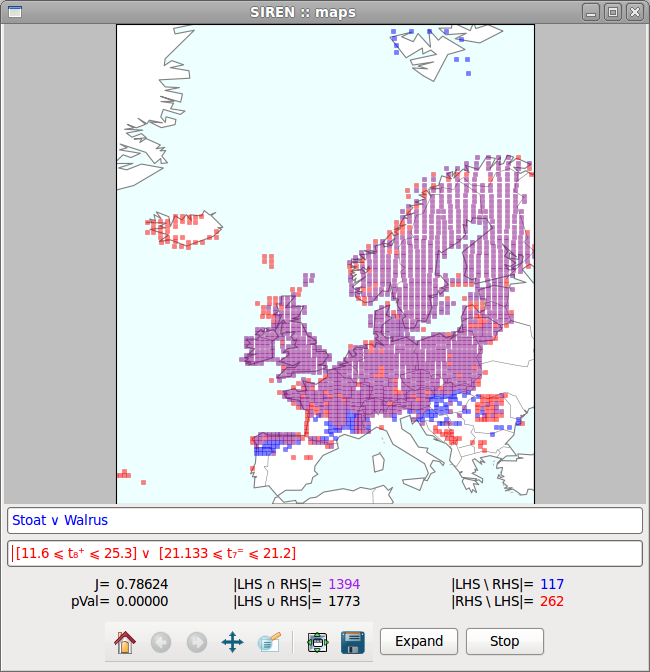
\includegraphics[width=.5\textwidth]{screenshots/siren_map.png}
%   \caption{Map panel, displaying a redescription on a map.}
%   \label{fig:map_panel}
% \end{figure}

\begin{figure*}[t]
  \centering
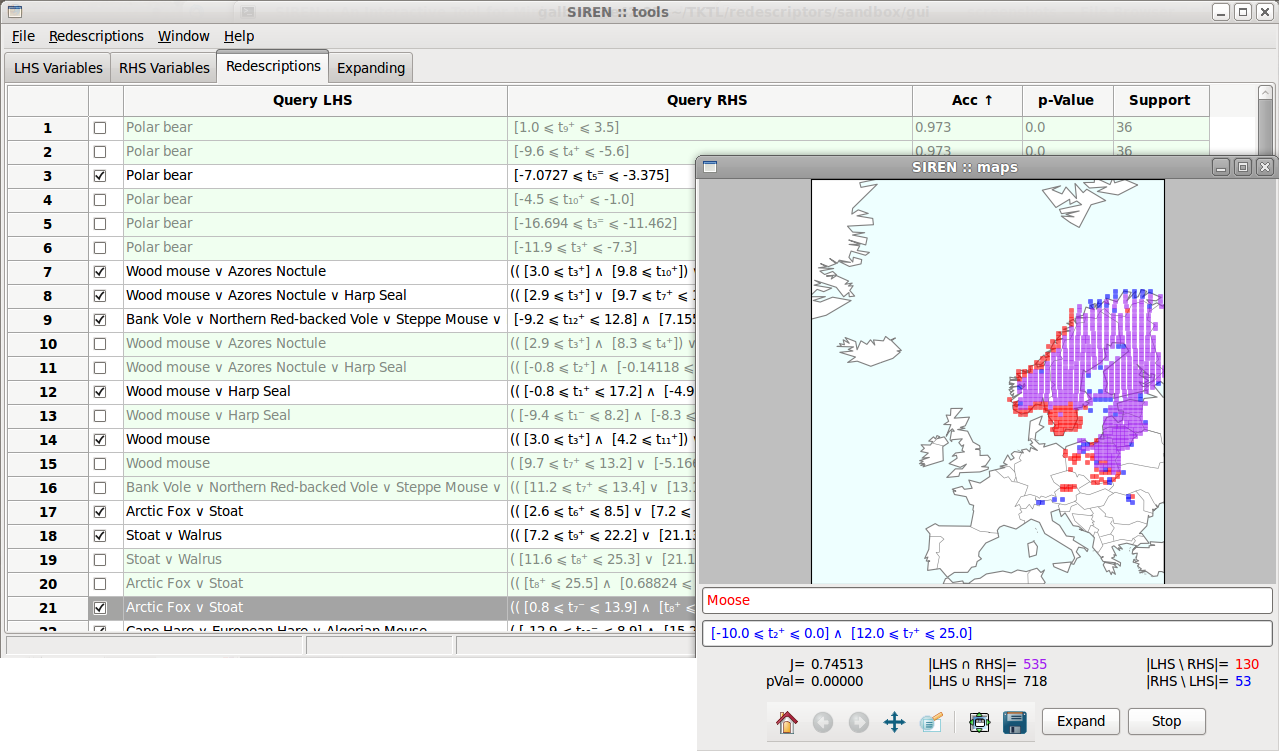
\includegraphics[width=\textwidth]{screenshots/both_panels_02.png}
  \caption{The \Siren\ interactive mining tool. The panel in the background displays a list of mined redescriptions. The foreground panel contains a plot of a selected redescription on a map, allowing edition and providing updated quality indicators.}
  \label{fig:both_panels}
\end{figure*}

\section{Sample applications}
For illustration purposes we selected two example datasets which
demonstrate the use of \Siren\ in different application domains.  The
first application is bioclimatic niche-finding while the second example
pertains the exploration of socio-economic statistics.

\prg{Biological niche-finding} 
An important problem in biology, known as \emph{niche-finding}, is a
particular instance of redescription mining.  The bioclimatic
constraints that must be met for a certain species to survive
constitute that species' bioclimatic envelope, or
niche~\cite{grinnell17niche}.  Finding such envelopes can help, e.g.\
to predict the results of global warming~\cite{pearson03predicting}.
A number of methods, involving regression, neural networks, and
genetic algorithms (see~\cite{soberon05interpretation}) have been
developped over the past ten year to model the bioclimatic envelope,
\textsc{BIOMOD}~\cite{thuiller09biomod} being a good example of a
modelling tool used in this domain.  But to the best of our knowledge,
none of these methods allows automatically finding both the set of
species and their envelope.

We give an example of the application of \Siren\ on this task using data
that describes spatial areas of Europe, squares of side roughly 50
kilometers.  The left hand side data contains information about the
mammals that live in these areas, while the right hand side consists
of bioclimatic variables\footnote{The data comes from two publicly available
datasets: European mammal atlas~\cite{mitchell-jones99atlas} and
Worldclim climate data~\cite{hijmans05very}.}.

\prg{Socio-economic statistics exploration}

% \begin{figure}
%   \centering
% 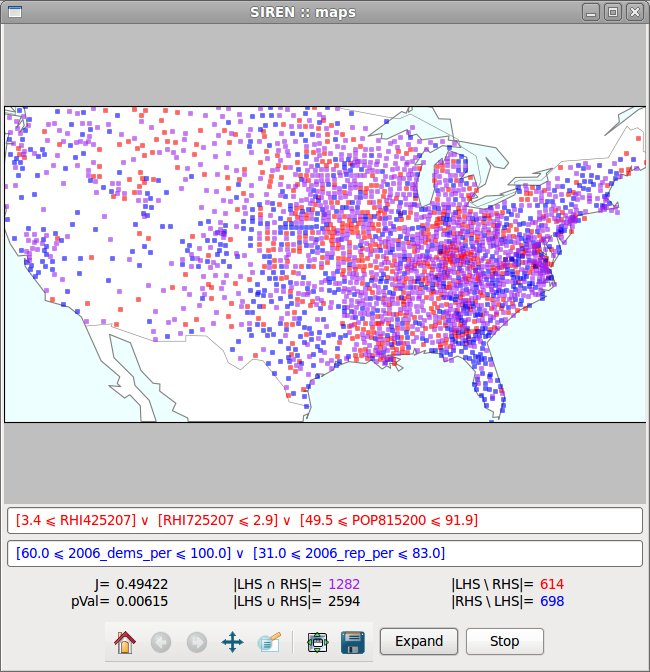
\includegraphics[width=.5\textwidth]{screenshots/siren_map_us_00.jpg}
%   \caption{Map panel, displaying a redescription on a map.}
%   \label{fig:map_panel}
% \end{figure}

To demonstrate the flexibility of the \Siren\ mining tool, we illustrate its usage on
an application from an entirely different domain, the exploration of socio-economic statistics. This time the data describes the counties
of continental United-States.  The left hand side data
contains socio-economic indicators about the counties, such as
population, age distribution or educational attainment. The right hand
side consists of data about funding of the electoral campaigns in
2006, 2008 and 2010\footnote{The data has been gathered from two public
websites: FedStats (\url{http://www.fedstats.gov/}) and Open
Secrets (\url{http://www.opensecrets.org/elections/}).}.


\section{Use-case scenario}
\label{sec:scenarios}
We exemplify the usage of \Siren\ by going through a generic workflow of
mining geospatial redescriptions.  A screenshot of the system,
displaying a list of redescriptions with one
particular redescription plotted on a map is shown in
Figure~\ref{fig:both_panels}.

\prg{Initial redescription mining}
Given the data, a natural first step is to use a redescription mining
algorithm to find the initial set of redescriptions. 

When the initial set of redescriptions is mined, starts the
interaction with \Siren.  The user is able to visualize the initial results,
edit, filter and refine them.  He can study the interesting
redescriptions plotted on a map, and compare several redescriptions by
visualizing them side by side. Uninteresting redescriptions can be
manually disactivated.
 
\prg{Extending a redescription} 
Sometimes the user wants to focus only on one of the queries in the
redescription, on some particular variable of interest or on part of
an existing redescription.  \Siren\ allows the user to automatically
extend a given redescription, i.e.\ let the algorithm add new literals
to the queries to make the redescription as accurate as possible.
% (see Fig.~\ref{fig:extending}). 

The extension mechanism of \Siren\ is based on the beam search
implemented in the \ReReMi\ algorithm.  It can also be used to study
more specific alternative extensions to a redescription, that the beam
search might have discarded at some point of the search because they
were not the best extensions.

In the climatic niche-finding task, for instance, we might select the Southwestern Water Vole and look for best extensions starting from that single variable. The intermediate redescriptions
explored during the beam search are returned at each step. 
They can be compared as shown in Figure~\ref{fig:comparison}. Below is the best found extension, of accuracy $0.665$:
\begin{equation*}
\begin{array}{l}
\text{Southwestern Water Vole }\lor\text{ Gray Dwarf Hamster }\\[1mm]
\quad\lor\text{ Savi's Pine Vole }\lor\text{ Mediterranean Monk Seal}\\[3mm]
[11.2 \leq t_{Mar}^{max}] \land  [0.51 \leq t_{Jan}^{avg} \leq 11.333]\\[1mm]
\quad\land  [42.75 \leq p_{Oct}^{avg} \leq 131.81] \land [50.556 \leq p_{Nov}^{avg} \leq 176.75],
\end{array}
\end{equation*}

This redescription indicates that areas where any of the four
species lives correspond to areas where the maximum temperature in
March is above $11.2$ degrees Celsius, the average temperature in January
between $0.51$ and $11.333$ degrees Celsius and the average precipitations in
October and November included in the range $42.75$ to $131.81$ millimeters and $50.556$ to $176.75$ millimeters, respectively.


% (see Figure~\ref{fig:extending})
% \begin{figure}
%   \centering
% 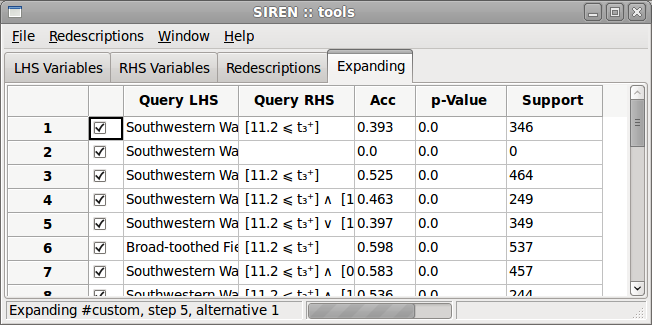
\includegraphics[width=0.5\textwidth]{screenshots/extending.png}
%   \caption{Tool panel. Intermediates results found during the extension of a redescription.}
%   \label{fig:extending}
% \end{figure}

\begin{figure}
  \centering
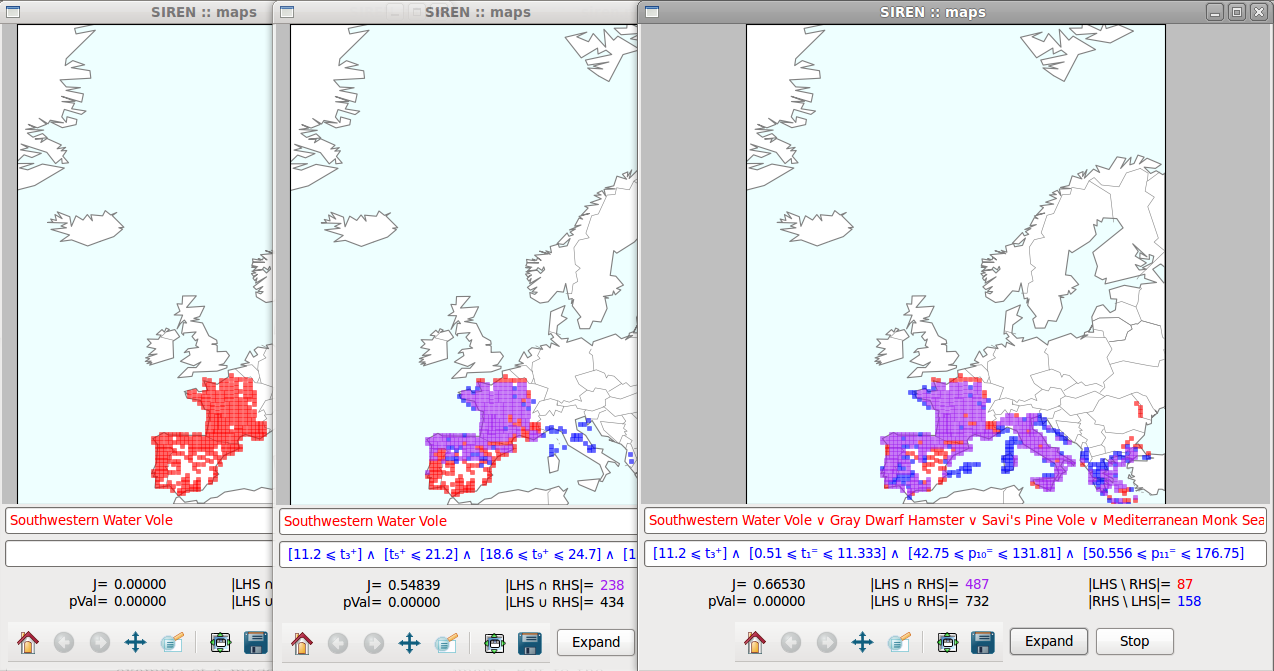
\includegraphics[width=0.45\textwidth]{screenshots/comparison.png}
  \caption{Several map panels. Comparing intermediate extensions automatically generate for a chosen starting variable. Red, blue and purple represents areas where only the left hand side query holds, only the right hand side query holds and where both queris hold, respectively.}
  \label{fig:comparison}
\end{figure}

\prg{Editing a redescription} 
It is typical that the algorithm returns redescriptions which the user
wants to edit. For example, some redescriptions might be overly
complex, or have exceedingly accurate boundaries for numerical
variables. The user can easily select the redescription he wants to
modify, open it in a map window and start editing it. He is able to
modify boundaries, add or remove literals. \Siren\ updates the map and
important statistics (accuracy, $p$-value, etc.) of the redescription,
allowing the user to see the effects of his modifications
immediately. This makes it easy for the user to check, e.g.\ whether
the new redescription would still be acceptably accurate.

Continuing with our example above, we might want to reduce the precision of the climatic constraints to integers. We could edit the query as follows
\begin{equation*}
\begin{array}{l}
[11 \leq t_{Mar}^{max}] \land  [0 \leq t_{Jan}^{avg} \leq 12]\\[1mm]
\quad\land  [42 \leq p_{Oct}^{avg} \leq 132] \land [50 \leq p_{Nov}^{avg} \leq 177],
\end{array}
\end{equation*}
and obtain a redescription with the slightly decreased accuracy of $0.659$.

\prg{Using subsets of variables}
Finally, a set of redescriptions might contain the same pair of
variables. This can happen, e.g.\ when these two variables are highly
correlated. The user, however, might want to see redescriptions that have
only one of these variables, not both. \Siren\ makes this simple: the user
only has to select a redescription, remove the variable he does not
want from the redescription, unselect it from the list of variables, and
extend the redescription. \Siren\ will not use the unselected
variables when extending or mining redescriptions.

Alternatively, in our running example, we might want to force
the algorithm to search alternative redescriptions that do not involve
any monthly precipitations. For that purpose, we simply unselect all such
variables before running the expansion anew. We will obtain the best
extensions containing only temperatures in the bioclimatic query, such as the following redescription of accuracy $0.653$

\begin{equation*}
\begin{array}{l}
\text{Southwestern Water Vole }\lor\text{ Cape Hare }\\[1mm]
\quad\lor\text{ Savi's Pine Vole }\lor\text{ Mediterranean Monk Seal}\\[3mm]
( [11.2 \leq t_{Mar}^{max}] \land  [20.1 \leq t_{Jul}^{max} \leq 32.9]\\[1mm] 
\quad\land  [0.51 \leq t_{Jan}^{avg} \leq 11.333]) \lor  [34.0 \leq t_{Aug}^{max}].
\end{array}
\end{equation*}

Note that this redescription was not returned previously since the
beam search focused on better ones involving precipitation variables.

% \begin{figure}
%   \centering
% 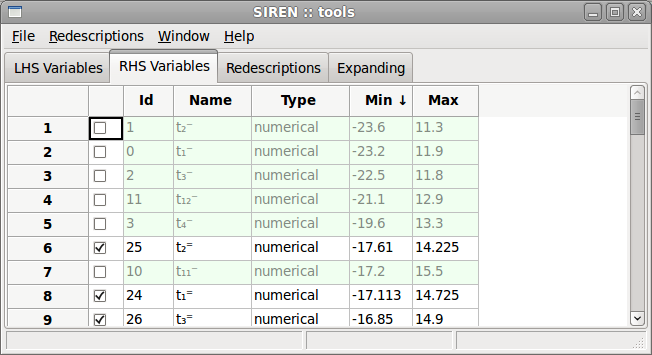
\includegraphics[width=.5\textwidth]{screenshots/variables_05.png}
%   \caption{Tool panel, uselecting variables.}
%   \label{fig:map_panel}
% \end{figure}

% \begin{figure}
%   \centering
% 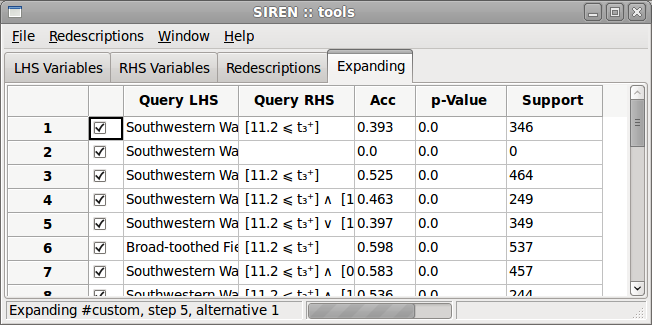
\includegraphics[width=0.5\textwidth]{screenshots/extending.png}
%   \caption{Tool panel, extending a redescription.}
%   \label{fig:extending}
% \end{figure}


\prg{Filtering redundant redescriptions}
\label{sec:filt-redund-redescr}
It is common to see a set of redescriptions that cover approximately
the same area even if they have (somewhat) different sets of
variables.  Indeed, redescriptions belong to the family of local
patterns, with each individual pattern independently describing
subsets of the data. Mining local patterns typically returns redundant
results that require filtering.  In such cases it is important to be
able to recognise and remove redundant redescriptions, i.e.\
redescriptions that do not convey significant new information, lest
the user be overwhelmed with the number of found
redescriptions. Again, \Siren\ allows automatic filtering of redundant
redescriptions. The user can either select a redescription and ask
\Siren\ either to filter out all redescriptions that are redundant
with respect to the selected one, or to go throught the whole list of
redescriptions filtering out all redescriptions that are redundant
with respect to some earlier-encountered (i.e.\ better)
redescription. Naturally, the user can revert the decisions made by
\Siren\ whenever he wants.

For instance, the results returned during the above extension
mentioned previously may contain many redundant redescriptions found
at different steps. We can easily sort them, e.g.\ by accuracy, select
one of interest and filter all the result down the list redundant with respect to it.

% \begin{figure}
%   \centering
% 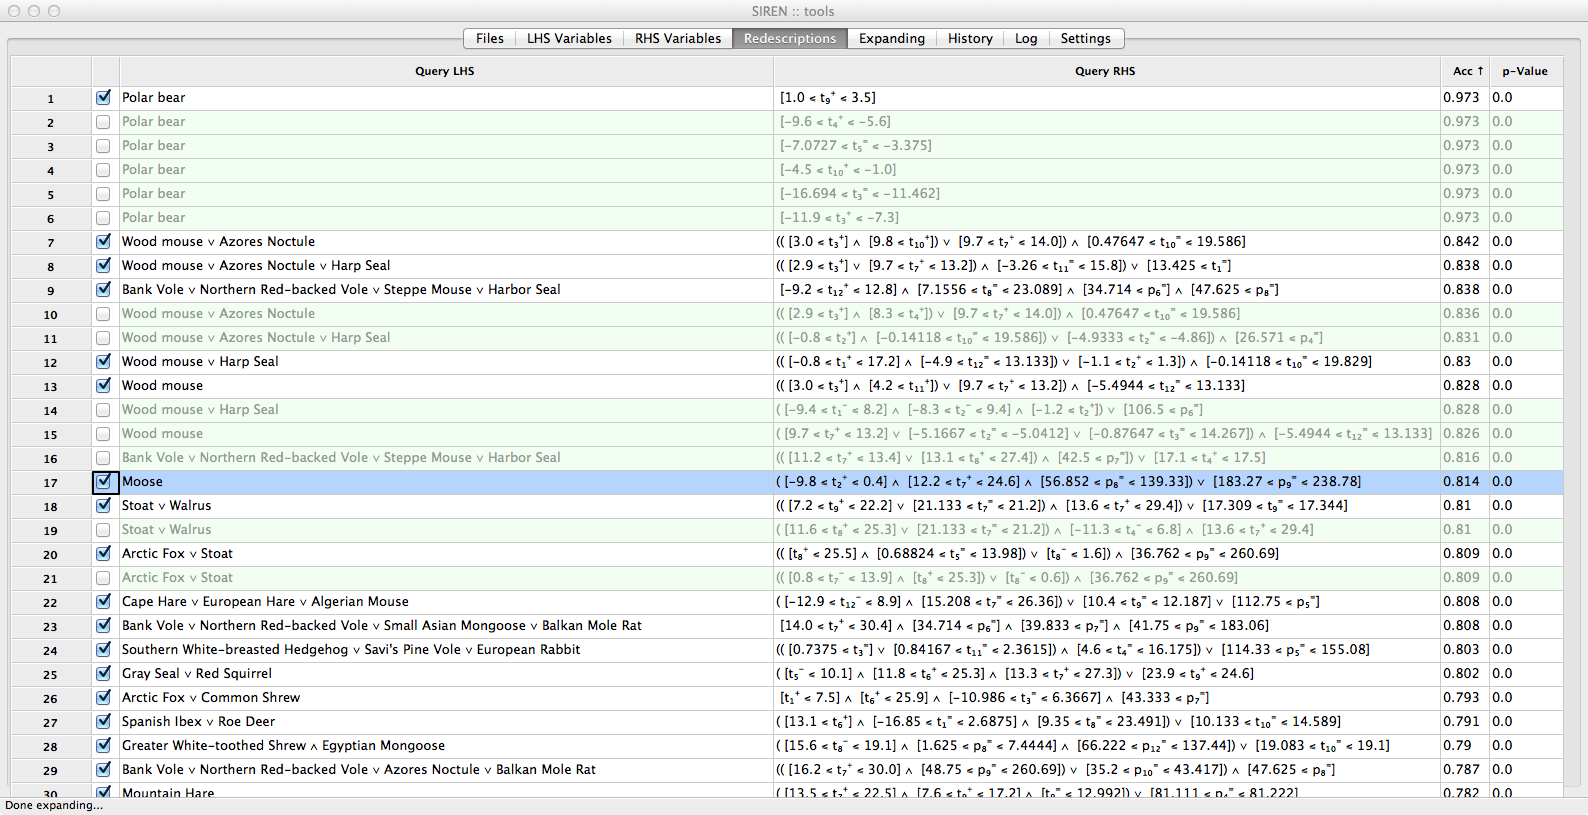
\includegraphics[width=.5\textwidth]{screenshots/redescriptions.png}
%   \caption{Tool panel, filtering redescriptions.}
%   \label{fig:filtering}
% \end{figure}

\prg{Outputting the results}
\label{sec:outputting-results}
Finally, \Siren\ facilitates the distribution of the results:
redescriptions can be exported in easy-to-read format and the
maps associated to redescriptions can be easily converted to
publication-ready graphics. 

\section{Redescription Mining}
Redescription mining aims at simultaneously finding multiple
descriptions of a subset of entities which is not previously
specified.  This is in constrast with other methods like Emerging
Patterns Mining (EPM), Contrast Set Mining (CSM) or Subgroup Discovery
(SD) (see \cite{kralj09supervised} for a unifying survey) or general
classification methods, where target subsets of entities are specified
via labels.  Currently, redescription mining is a purely descriptive
approach, its predictive power remains to be explored.  Since its
introduction in~\cite{ramakrishnan04turning} various algorithms have
been proposed for Boolean redescription mining, based on approaches
including decision
trees~\cite{ramakrishnan04turning,kumar07redescription},
co-clusters~\cite{parida05redescription}, and frequent
itemsets~\cite{gallo08finding}.

At the core of \Siren\ is the \ReReMi\ redescription mining
algorithm. This greedy algorithm uses an efficient on-the-fly
discretization technique to extend redescription mining to categorical
and numerical variables.  Below, we give an outline of the concepts and
algorithms involved. Full details can be found
in the original publication~\cite{galbrun11black}.

We consider Boolean, categorical, and numerical variables. Boolean
variables can be interpreted as a truth value assignment in a natural
way.  For a real-valued variable $v$ truth value assignments are
induced by relations $[a \leq v \leq b]$ and $[v=c]$, respectively,
where $[a, b]$ is an interval and $c$ some category.  These truth
assignments and their negations constitute \emph{literals} which can
be combined using the Boolean operators $\land$ (and) and $\lor$ (or)
to form \emph{queries}.  Then, a redescription is simply a pair of
queries over variables from the two sets.  The support of a query, is
the subset of entities for which the query holds true.  The
\emph{accuracy} of a redescription is measured by the \emph{Jaccard
  coefficient} of the supports of its two queries. We compute
\pValue{}s, indicating how likely it is to observe such an overlap for
independent queries, which can be used to discard uninteresting
redescriptions.

% The search space of all Boolean formulae is too huge to be manageable.
% Therefore, we need to restrict ourselves to a subset of formulae that
% provides a good compromise between expressive power, difficulty of the
% search, and interpretability.
% For this purpose, we consider queries that can be parsed in linear
% order, without trees, and allow every variable to appear only once.
% For example, $(a \lor b) \land \lnot c$ is an acceptable query, but
% $(a \land b) \lor (c \land d)$ is not. Yet, the search space remains
% exponential and we still resort to a heuristic pruning during the
% search.
We use a strategy similar to beam-search to explore the
solution space.  The basic idea is to construct queries bottom-up,
starting from singleton redescriptions (i.e.\ both queries contain
only one literal) and progressively extending them by appending
operators and literals. %  For example, we could start with a pair $(a,
% \lnot b)$, and try to extend it to $(a\land c, \lnot b)$, $(a \lor c,
% \lnot b)$, $(a \land \lnot c, \lnot b)$, etc.
After evaluating all
possible one-step extensions, we select the best candidates and extend
them in turn. This process stops when no new redescription can
be generated.

% We exploit some
% simple observations to make the computation of accuracy more
% efficient. This allows to evaluate candidates faster, especially
% extensions with non-Boolean variables.
% We compute a \pValue{} that represents the probability that two random
% queries with marginal probabilities (i.e.\ the fraction of entities
% supporting them) equal to those of $q_\iLHS$ and $q_\iRHS$ have an
% intersection equal to or larger than $\abs{\supp(q_\iLHS,
%   q_\iRHS)}$. This probability uses the binomial distribution. The higher the
% \pValue, the more likely it is to observe such a support for
% independent queries, and the less significant the query. Redescriptions with too high \pValue{} can be discarded.

\section{Implementation details}
\Siren\ and \ReReMi\ are implemented in Python.  The interface is built
with the \texttt{wxPython} Open Source GUI toolkit, ensuring
cross-platform compatibility.  The \texttt{matplotlib} library enables
to generate high quality figures seamlessly integrated in the
interface.  \Siren\ allows for simple editing of the redescriptions thanks to flexible parsing of different representations. It can handle any data provided in a compatible
format.

The formulation of redescription mining presented here assumes that
the describing variables are apriori partitioned into two sets, and
looks for a pairs of queries over these two sets, respectively.
However, this can be naturally adapted to settings with a single set
of describing variables.  One might then search for pairs of queries,
with the constraint that the two subsets of variables appearing in the
queries of any redescription be disjoint or enable the user to
interactively determine the split between the variables.

\section{Conclusions}
We present \Siren, a tool mining geospatial redescriptions. It enables
users to interactively mine, edit and extend redescriptions. It also
features visualization of the redescriptions on a map, a key to the
interpretation of the results of geospatial data mining.

We will give the chance to the public to experiment with \Siren\ and
together consider how this tool could be used to explore their own geospatial
data and help answer their data analysis need.

\bibliographystyle{abbrv}
%\nocite{*}
\bibliography{bibsiren}  
\balancecolumns

% That's all folks!
\end{document}

%%% Local Variables: 
%%% mode: latex
%%% TeX-master: t
%%% End: 
